\begin{figure}[htbp]
\centering
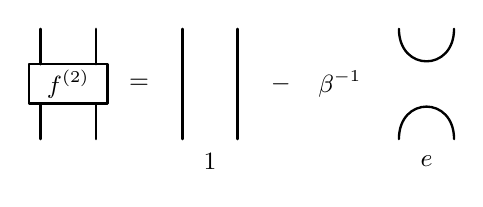
\begin{tikzpicture}[
  x=1cm,y=1cm,line width=0.85pt,
  line cap=round,line join=round,font=\small]
  % First row: the projector, identity, and cup--cap operator.
  % Each diagram has two inputs at y=0 and two outputs at y=1.4.
  \draw (0,0)--(0,0.45);
  \draw (0.7,0)--(0.7,0.45);
  \draw (0,0.95)--(0,1.4);
  \draw (0.7,0.95)--(0.7,1.4);
  \draw (-0.15,0.45) rectangle (0.85,0.95);
  \node at (0.35,0.7) {$f^{(2)}$};

  \node at (1.25,0.7) {$=$};
  \draw (1.8,0)--(1.8,1.4);
  \draw (2.5,0)--(2.5,1.4);
  \node at (2.15,-0.28) {$1$};

  \node at (3.05,0.7) {$-$};
  \node at (3.8,0.7) {$\beta^{-1}$};
  % Lower cap joins the two input endpoints; upper cup joins outputs.
  \draw (4.55,0)
    .. controls (4.55,0.55) and (5.25,0.55) .. (5.25,0);
  \draw (4.55,1.4)
    .. controls (4.55,0.85) and (5.25,0.85) .. (5.25,1.4);
  \node at (4.9,-0.28) {$e$};
\end{tikzpicture}

\smallskip

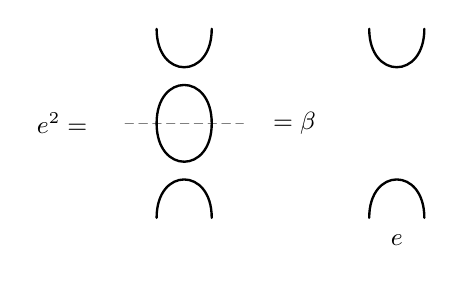
\begin{tikzpicture}[
  x=1cm,y=1cm,line width=0.85pt,
  line cap=round,line join=round,font=\small]
  % Second row: stack two e diagrams. Their common boundary is y=1.2.
  % The two middle arcs form one closed loop after gluing.
  \node at (0,1.2) {$e^2=$};
  \draw[gray,densely dashed,line width=0.4pt]
    (0.8,1.2)--(2.3,1.2);
  \draw (1.2,0)
    .. controls (1.2,0.65) and (1.9,0.65) .. (1.9,0);
  \draw (1.2,1.2)
    .. controls (1.2,0.55) and (1.9,0.55) .. (1.9,1.2)
    .. controls (1.9,1.85) and (1.2,1.85) .. (1.2,1.2)
    --cycle;
  \draw (1.2,2.4)
    .. controls (1.2,1.75) and (1.9,1.75) .. (1.9,2.4);

  \node at (2.95,1.2) {$=\beta$};
  % The surviving cup--cap has the same four exterior endpoints.
  \draw (3.9,0)
    .. controls (3.9,0.65) and (4.6,0.65) .. (4.6,0);
  \draw (3.9,2.4)
    .. controls (3.9,1.75) and (4.6,1.75) .. (4.6,2.4);
  \node at (4.25,-0.28) {$e$};
\end{tikzpicture}
\caption{The two-strand Jones--Wenzl projection, with checkerboard
shading suppressed. Morphisms are read from bottom to top, and
$\beta=\sqrt{[M:N]}$. The normalized Jones projection is
$e/\beta$. In the lower row the dashed line marks the
glued boundary of two copies of $e$. The resulting internal loop
evaluates to $\beta$, leaving the cup--cap operator and proving
$e^2=\beta e$.}
\label{fig:EH-jones-wenzl-two}
\end{figure}
